\section{The Proposed Approach}
	\label{sec:propApproach}
	\subsection{Signals database}
		\par To conduct this research, a series of voices were collected in the vicinity of the Institute of Biosciences, Languages and Exact Sciences (IBILCE) at UNESP in São José do Rio Preto, in the state of São Paulo. Samples were collected from 21 individuals, of which 20 were used since, in one case, it was not possible to collect all the necessary data. Such recordings consist of digits in a range of 0 to 9 spoken both in English and in Portuguese. The announcers were chosen according to their sex and age so that the studied sample has coverage that includes people from pre-school children to adults between 50 and 60 years of age, males and females.
		
		\par The recordings were made using an Asus smartphone model \textit{Ze550kl} running the operating system \textit{Android 6.0.1} in different environments with various noise levels in the background, ensuring a good variability of common interferences, characterizing real cases. Files were used in the format \textit{wave} without compression with quantization of 16 bits and a sampling rate of 44100Hz, allowing, according to the Nyquist theorem, frequencies up to 22050Hz to be recorded.
		
		\par Once the signals were collected, the digits pronounced in them were separated one by one using a tool developed for this purpose, resulting in a total of 410 voice signals of different time durations that were labeled ``genuine''. For each of them, a ``mirror'' signal was created, re-recorded by a second device, an notebook \textit{Acer} model \textit{Travelmate B} with the operating system \textit{Arch GNU/Linux}, featuring the 410 signals labeled as  ``spoofed''.
		
	\subsection{Organization of the signals database}
		\par The database organization took place by type, that is, genuine or spoofed, language, digit dictated, and interlocutor considered. A hierarchical directory structure was created to allow easy and intuitive access to each of the \textit{wav} files, whether by automated means or not. The spoofed files reside in the ``playback'' directory, while the genuine ones are in the ``live'' directory. This organization is illustrated in Figures \ref{fig:directorystructlevel01}, \ref{fig:directorystructlevel02} and \ref{fig:directorystructlevel03}.		
		\begin{figure}[ht]
			\centering
			\subfloat[0.33\textwidth][Database level 1]{
				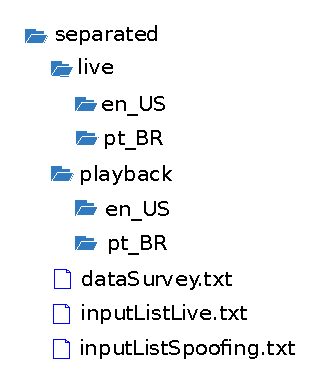
\includegraphics[height=132px]{../00-dissertation/monography/images/directoryStructLevel01.pdf}
				\label{fig:directorystructlevel01}
			}
			\subfloat[0.33\textwidth][Database level 2]{
				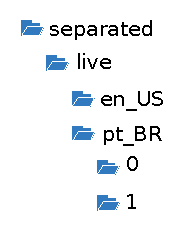
\includegraphics[height=83px]{../00-dissertation/monography/images/directoryStructLevel02.pdf}
				\label{fig:directorystructlevel02}
			}
			\subfloat[0.33\textwidth][Database level 3]{
				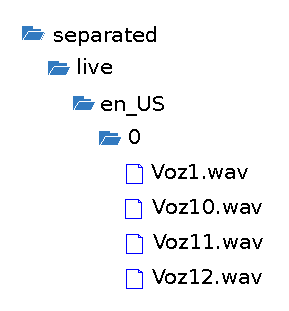
\includegraphics[height=100px]{../00-dissertation/monography/images/directoryStructLevel03.pdf}
				\label{fig:directorystructlevel03}
			}
			\caption{Database organization}
			\label{fig:directorystructlevel010203}
		\end{figure}
		
		\par To facilitate automation of processing, it was created three text files:
		\begin{itemize}
			\item \textit{\textbf{dataSurvey.txt}}: Contains age, sex data along with a file name generated for each interviewee;
			\item \textit{\textbf{inputListLive.txt}}: A list of paths for all genuine files;
			\item \textit{\textbf{inputListSpoofing.txt}}: A list of paths for all spoofed files.
		\end{itemize}
	
		\par Just to illustrate, the directory contents of the \textbf{``separated \textfractionsolidus live \textfractionsolidus en\_US \textfractionsolidus 0''} consists of several \textit{wave} files, each identifying the speaker to which it belongs as shown in Figure \ref{fig:directorystructlevel03}.
	
	\subsection{Proposed approach structure}
		\par The proposed strategy to differentiate genuine voice signals from the spoofed ones occurred as illustrated in Figure \ref{fig:propApproachStruct}. In particular, the methodology consists in obtaining the raw data of all 410 + 410 = 820 genuine and spoofed voice signals, followed by the conversion of each of them to a corresponding feature vector, as explained below. Subsequently, the best subsets of characteristics were chosen based on Paraconsistent Engineering. Continuing, random separations between the feature vectors, with different proportions, were performed to isolate those destined for classifier training/modeling from those destined for classification tests. Finally, the tests performed and the results are shown in the next Section.
		
		\begin{figure}[h]
	\centering
	\caption{Estrutura da estratégia proposta}
	\scalebox{0.75}	{
		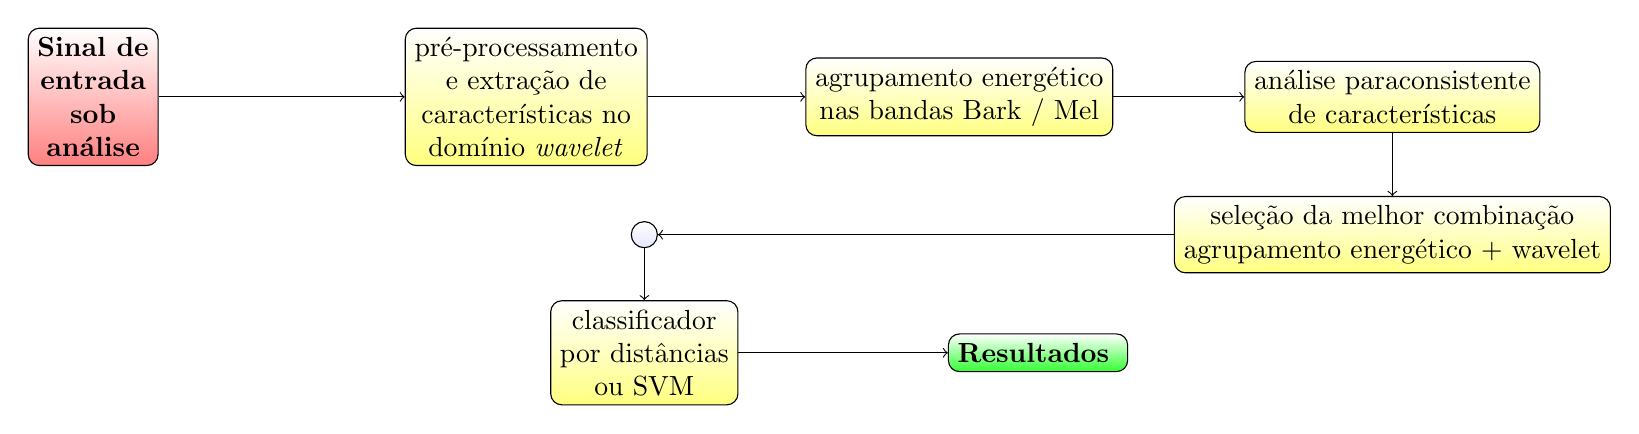
\begin{tikzpicture} 
			\node (z1)[shape=rectangle, rounded corners, draw, align=center, top color=white, bottom color=red!50] 
			at (0,2){
				\textbf{Sinal de} \\ \textbf{entrada} \\ \textbf{sob} \\ \textbf{análise}
			}; 
				
			\node (z2)[shape=rectangle, rounded corners, draw, align=center, top color=white, bottom color=yellow!50] 
			at (5.5,2){
				pré-processamento \\ e extração de \\ características no \\ domínio \textit{wavelet}
			}; 	
			
			\node (z3)[shape=rectangle, rounded corners, draw, align=center, top color=white, bottom color=yellow!50] 
			at (11,2){
				agrupamento energético \\ nas bandas Bark / Mel
			}; 	
			
			\node (z4)[shape=rectangle, rounded corners, draw, align=center, top color=white, bottom color=yellow!50] 
			at (16.5,2){
				análise paraconsistente \\ de características
			}; 
			
			\node (z5)[shape=rectangle, rounded corners, draw, align=center, top color=white, bottom color=yellow!50] 
			at (16.5,0.25){
				seleção da melhor combinação \\ agrupamento energético + wavelet
			}; 
					
			\node (z6)[shape=circle, draw, align=center, top color=white, bottom color=blue!10] 
			at (7,0.25) {};
			
			\node (z7)[shape=rectangle, rounded corners, draw, align=center, top color=white, bottom color=yellow!50] 
			at (7,-1.25) {
				classificador \\ por distâncias \\ ou SVM
			};
			
			\node (z8)[shape=rectangle, rounded corners, draw, align=center, top color=white, bottom color=green!80] 
			at (12,-1.25) {
				\textbf{Resultados}
			};
			
			\path[->] (z1) edge (z2);
			\path[->] (z2) edge (z3);
			\path[->] (z3) edge (z4);
			\path[->] (z4) edge (z5);
			\path[->] (z5) edge (z6);
			\path[->] (z6) edge (z7);	
			\path[->] (z7) edge (z8);
		\end{tikzpicture}
	}
	\label{fig_arq}
	\\Fonte: Elaborado pelo autor, 2021.
\end{figure}
		
		\par As mentioned in the previous sections, the feature vectors of this approach were obtained based on the \textit{Wavelet} Transform, converting the voice signals from the time domain to the time-frequency domain. In particular, in the experiments detailed below, the following \textit{wavelet} filters were tested: Haar, Daubechies with support from 4 up to 76, Symmlets with supports 8, 16 and 32, Coiflets with supports 6, 12, 18, 24 and 30, Beylkin with support 18 and Vaidyanathan with support 24.

	\subsection{Procedures}
	
		\par To guarantee the comparison with other works, it was necessary to adopt several ways of representing the corresponding results for each experimental configuration:
	
		\begin{itemize}
			\item Confusion table.
			\item Accuracy and its respective standard deviation.
			\item EER (Equal Error Rate).
		\end{itemize}
	
		\par In the confusion table example \ref{tab:confusionMatrixSample}, the \textbf{lines} represent the \textbf{estimated classes} and the \textbf{columns} the \textbf{true classes}, where:

		\begin{itemize}
			\item \textbf{TP}: Quantity of true items classified as such (\textit{True Positive}).
			\item \textbf{TN}: Quantity of false items classified as such (\textit{True Negative}).
			\item \textbf{FN}: Quantity of true items classified as false (\textit{False Negative}).
			\item \textbf{FP}: Quantity of false items classified as true (\textit{False Positive}).
		\end{itemize}

		\begin{table}
\newcommand{\mc}[3]{\multicolumn{#1}{#2}{#3}}
\definecolor{tcB}{rgb}{0.447059,0.74902,0.266667}
\definecolor{tcC}{rgb}{0,0,0}
\definecolor{tcD}{rgb}{0,0.4,0.701961}
\definecolor{tcA}{rgb}{0.65098,0.65098,0.65098}
\begin{center}
	\begin{tabular}{ccc}
		% use packages: color,colortbl
		\mc{1}{l}{} & \mc{1}{>{\columncolor{tcA}}c}{\textbf{Verdadeiro}} & \mc{1}{>{\columncolor{tcA}}c}{\textbf{Falso}}\\

		\mc{1}{>{\columncolor{tcA}}r}{\textbf{Verdadeiro}} & \mc{1}{>{\columncolor{tcB}}c}{\textcolor{tcC}{VV}} & \mc{1}{>{\columncolor{tcD}}c}{\textcolor{tcC}{FV}}\\

		\mc{1}{>{\columncolor{tcA}}r}{\textbf{Falso}} & \mc{1}{>{\columncolor{tcD}}c}{\textcolor{tcC}{FF}} & \mc{1}{>{\columncolor{tcB}}c}{\textcolor{tcC}{VF}}
	\end{tabular}
	\caption{Exemplo de matriz de confusão}
	\label{tab:confusionMatrixSample}
\end{center}
\end{table}


		\par To be calculated the accuracy uses the values of \textit{TP}, \textit{TN} and the number of elements (\textit{N}) as shown in Equation \ref{eq:calculoDaAcuracia}.
		
		\begin{equation}
			accuracy = \dfrac{TP + TN}{N} \qquad.
			\label{eq:calculoDaAcuracia}
		\end{equation}

		\par In order to calculate the EER, the values of \textit{FP} and \textit{FN}  are taken into account \cite{ghazali2018recent}, from these values the \textit{False Acceptance Rate (\textbf{FAR})} is calculated as shown in the Equation \ref{eq:FAR} and \textit{False Rejection Rate (\textbf{FRR})} as shown in Equation \ref{eq:FRR}.

		\begin{equation}
			FAR=\dfrac{FP}{TN+FP} \qquad.
			\label{eq:FAR}
		\end{equation}
		
		\begin{equation}
			FRR=\dfrac{FN}{TP+FN} \qquad.
			\label{eq:FRR}
		\end{equation}

		\par Confusion tables are calculated for a sufficient number of times until \textbf{\textit{FAR} is equal to \textit{FRR}}, at each cycle the feature vectors are switched randomly so that different values are obtained, in this work some cases needed more than 12,000 iterations in order to find the configuration that made \textit{FAR=FRR}.

		\par At each iteration the values of FAR and FRR are stored in two vectors, one for each, so the vector belonging to FAR is sorted in ascending order and the other in decreasing order. These points drawn on the graph together with a line that divides the plane of the graph in half such that $x=y$ constitute what is conventionally called a \textit{Detection Error Trade off (DET)} graph.
		
		\par The effective value of \textbf{ERR is at the intersection of the line defined by x=y} with the curve defined by FAR and FRR, that is why the calculation of a single value as shown in Algorithm \ref{lst:EERAlgo} and Figure \ref{fig:eeralgo} because if $x=ERR$ then also $y=ERR$.
		
		\begin{lstlisting}[language=C++, caption={EER algorithm}, label={lst:EERAlgo}]
double shortestDistance = highestValue();
double currentDistance = -highestValue();

double coordinateAboveDiagonalLine = { 0, 0 };
double coordinateBellowDiagonalLine = { 0, 0 };

sortAscending(FARVector);
sortDescending(FRRVector);

for (i = 0; i < FARVector.size(); i++) {
	// Calculate the distance between the coordinates defined
	// by the FAR and FRR vectors and the line defined by x=y
	currentDistance = absoluteValue((FARVector[i] - FRRVector[i]) / squaredRoot(2));
	
	// Stores just the shortest distance above the x=y line
	if (currentDistance <= shortestDistance && FRRVector[i] >= FARVector[i]) {
		shortestDistance = currentDistance;
		coordinateAboveDiagonalLine[0] = FARVector[i];
		coordinateAboveDiagonalLine[1] = FRRVector[i];
		jumpToNextIteration();
	}

	// Stores just the shortest distance bellow the x=y line
	coordinateBellowDiagonalLine[0] = FARVector[i];
	coordinateBellowDiagonalLine[1] = FRRVector[i];
	
	breakLoop();
}

// Calculates the intersection point of the curve defined by the FAR and FRR points and the x=y line
y = coordinateAboveDiagonalLine[0] - coordinateBellowDiagonalLine[0] - 1;
x = coordinateBellowDiagonalLine[1] - coordinateAboveDiagonalLine[1] + 1;
c = coordinateAboveDiagonalLine[1] * coordinateBellowDiagonalLine[0] - coordinateAboveDiagonalLine[0] * coordinateBellowDiagonalLine[1];

// Calculates the equal error rate
EER = -(c / (x + y));
\end{lstlisting}
		
		\begin{figure}[H]
			\centering
			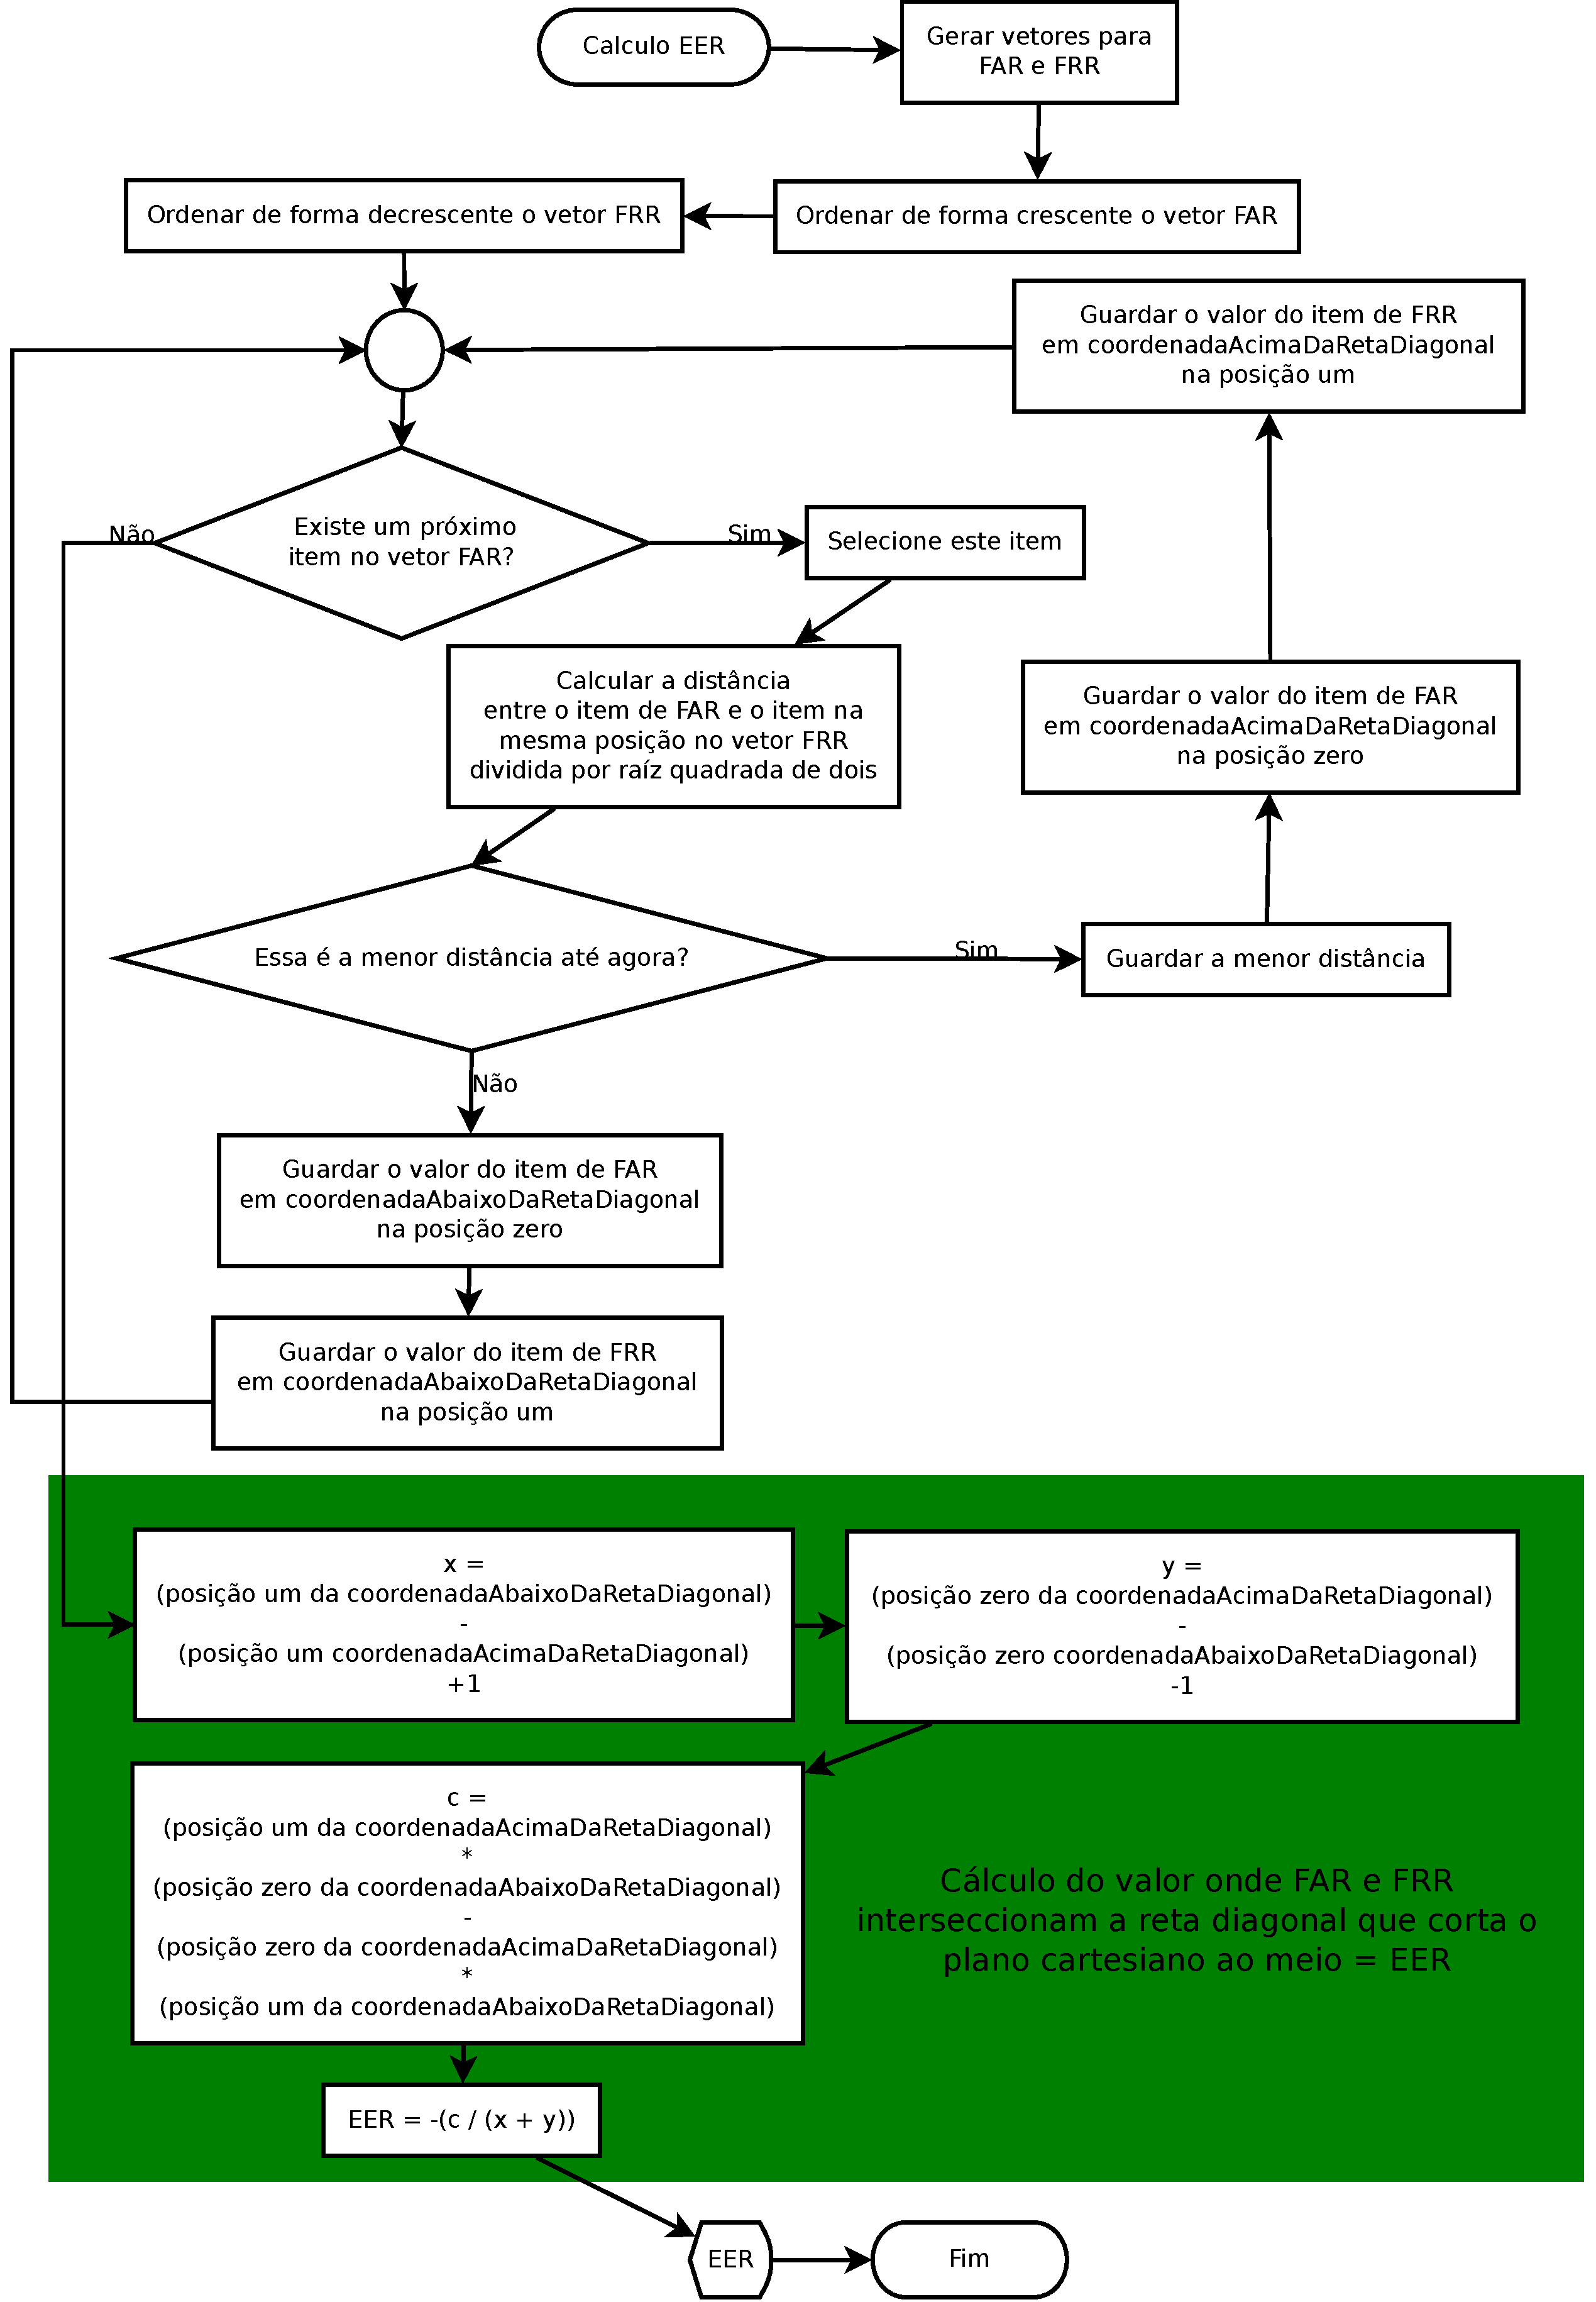
\includegraphics[angle=-90, width=1\linewidth]{images/EERAlgo.pdf}
			\caption{EER calculus algorithm}
			\label{fig:eeralgo}
		\end{figure}

		\subsection{Procedure 1: Bark and mel scales and \textit{wavelets} filters}
			\label{sec:propApproach:subsec:Experiment1}
			\par The objective of this procedure is to investigate, according to Paraconsistent Engineering, which of the combinations between BARK or MEL scales and the various \textit{wavelets} considered generate the most propitious feature vectors, that is, which attract the $point(G_1, G_2)$ to a position closer to the vertex $(1,0)$ of the paraconsistent plane.
			
			\par The \textit{packet-wavelet} transformations were performed, with the already mentioned filters (Haar, Daubechies, etc.), up to the maximum possible level, implying maximum resolution in frequency so that, after this, the samples of the transformed signals were grouped to correspond to the \textbf{spectral intervals} defined in the BARK and MEL scales. On that scale, the feature vectors were made up of 24 coefficients, differently, on this scale, the feature vectors were formed with 13 coefficients due to the derivation of the signal at the end of the generation process. The Algorithm \ref{lst:experiment01Algo} and the Figure \ref{fig:experiment01Algo} contains a description of such processes.
			
			\begin{lstlisting}[language=C++]
// Carregue para a memoria um dos conjuntos de amostra
for (listaDeAmostras : {listaComVoiceSpoofing, listaSemVoiceSpoofing}) {
	// Selecione o proximo tipo de wavelet
	for (wavelet : wavelets) {
		// Selecione entre BARK ou MEL
		for (barkOuMel : {BARK, MEL}) {
			// Selecione o proximo sinal dentro da amostra
			for (sinal : listaDeAmostras) {
				tamanhoOtimo=calcularTamanhoOtimo(sinal);
				redimensionar(sinal, tamanhoOtimo);
				sinalTransformado=wavelet(sinal, wavelet);
				energias=calcularEnergias(sinalTransformado, barkOuMel);
				energias=normalizar(energias);
				
				// Armazene os resultados
				resultados[wavelet.nome()][barkOuMel][listaDeAmostras.nome()].adicionar(energias);
			}
		}
	}
}
// Posicione os resultados no plano paraconsistente
mostraResultadosNoPlanoParaconsistente(resultados);
\end{lstlisting}
			
			\begin{figure}[H]
				\centering
				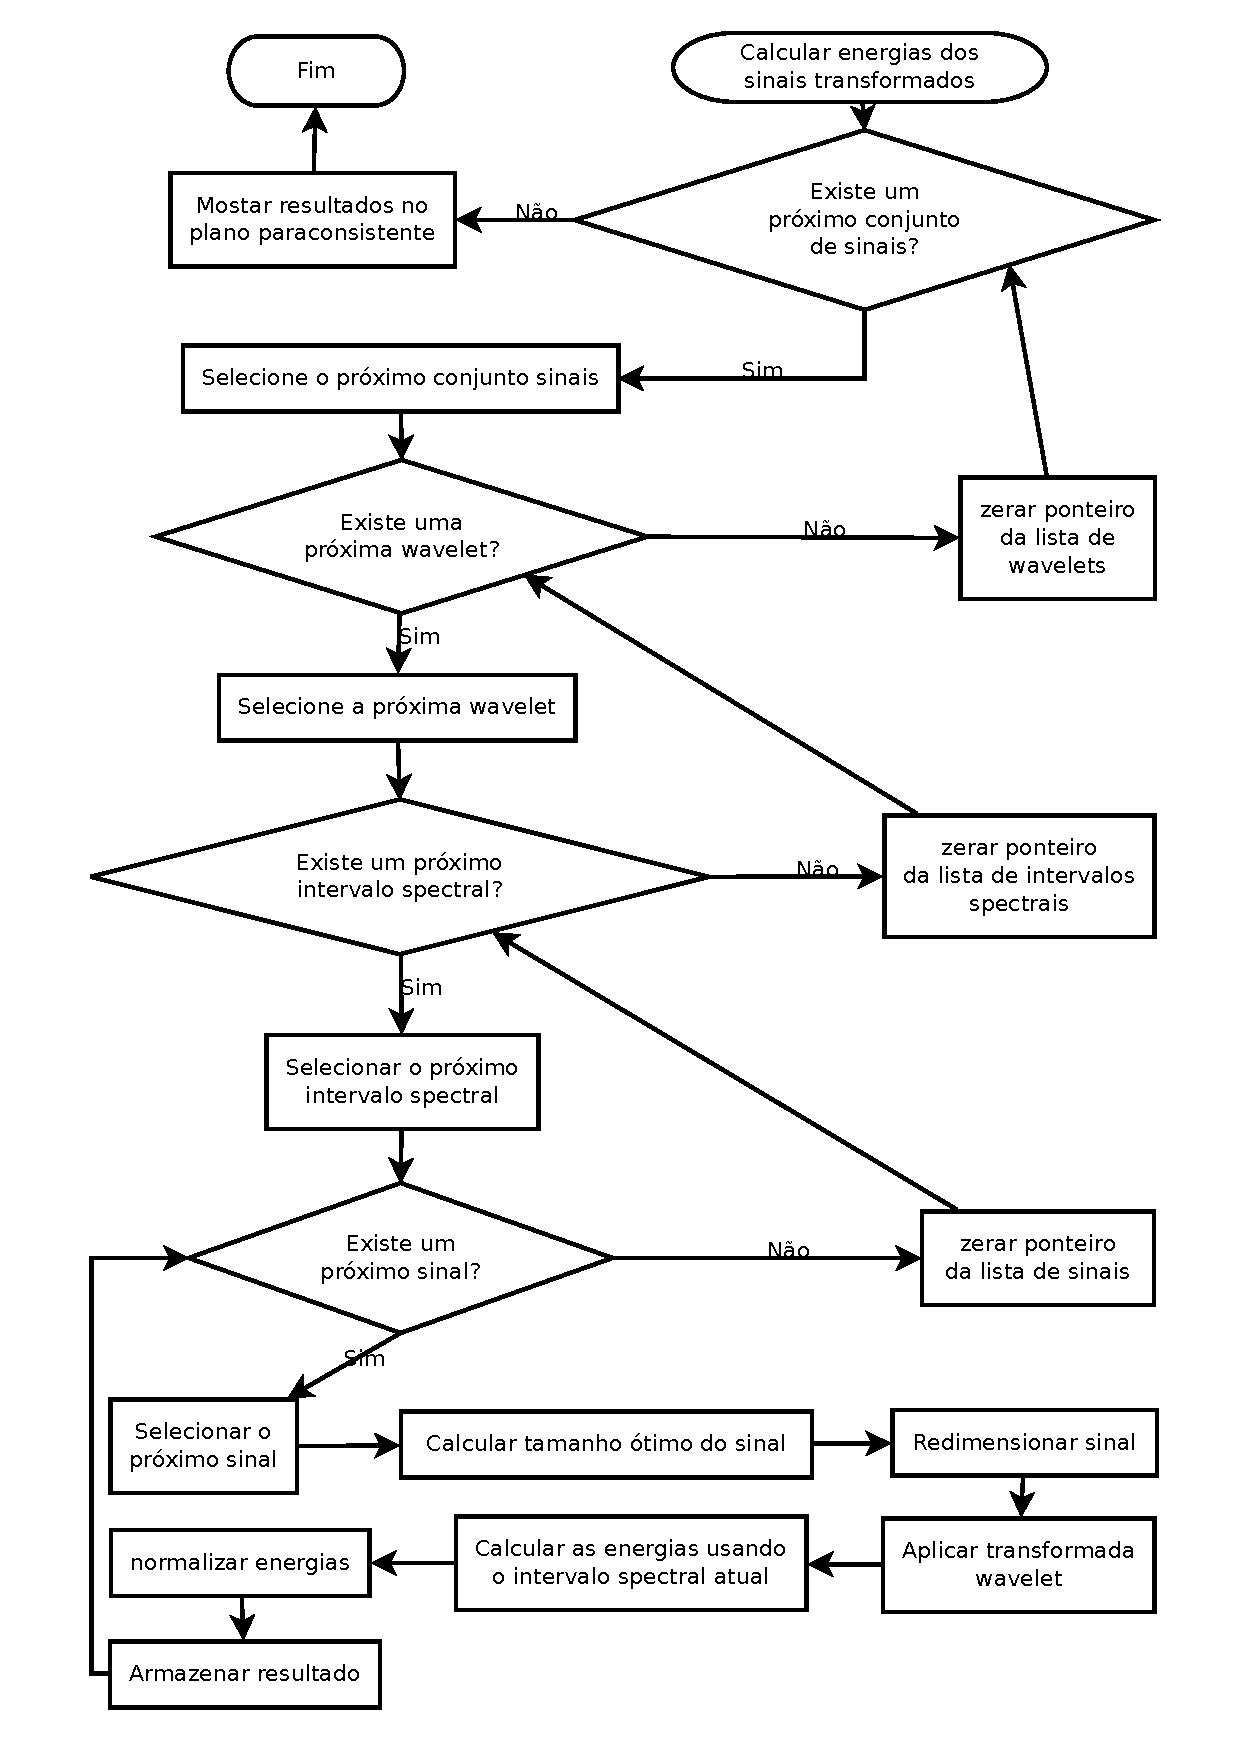
\includegraphics[angle=-90,width=1\linewidth]{images/AlgoProcedure01.pdf}
				\caption{Procedure 1 algorithm}
				\label{fig:experiment01Algo}
			\end{figure}
			
			\par It should be noted that, before applying the \textit{packet-wavelet} transformation, it was necessary to resize the signals so that the length fits in a power of 2 size, as indicated in the equation \ref{eq:optimalSize}. This is necessary to avoid loss of voice passages at the end of the transformed signal because the \textit{wavelet} transform performs an order 2 \textit{downsampling}, that is, at each level of decomposition the size of the signal vector is reduced in half. If the length is other than that mentioned, in some part of the process the division will not be integer, causing some signals samples to be lost.
			
			\par To adjust the voice signal size under analysis, the equation \ref{eq:optimalSize} was used, in which \textit{\textbf{proxInt}} is a function that returns the next integer of the real argument. For example, $proxInt(1.5)=2$.

			\begin{equation}
				optimalSize=2^{proxInt(\log_{2}size)}
				\label{eq:optimalSize}
			\end{equation} 
			
			\par After resizing the signal, the maximum level of transformations is given by Equation \ref{eq:maxWaveletTransf}. 
			
			\begin{equation}
				maxTrans=\log_{2}(size) \qquad.
				\label{eq:maxWaveletTransf}
			\end{equation}
			
		\subsection{Procedure 2 - distance based classification}
			\label{sec:propApproach:subsec:Experiment2}
			\par The purpose of this procedure is to verify, considering the best combinations discovered by the previous procedure, the accuracy of \textit{pattern-matching} classifier by Euclidean and Manhattan distances. At this stage, the feature vectors generated by procedure 1 are provided to the classifier for the appropriate measurements.
			
			\par In order to evaluate the behavior of classifier with multiple database proportions of 10\% up to 50\% for modeling, and the remainder for tests, it was defined that, for each proportion, the random draw for choosing the feature vectors, would be executed $n=t\cdot\frac{t+1}{2}$ times, with $t$ being the maximum number of tests that can be performed with a certain percentage of the vectors. In each of these runs, the vectors order within the samples, rewritten and genuine, was randomly switched.
			
			\par For each percentage, the best and worst accuracy were collected, as well as their respective confusion matrices and thus calculated their \textit{EERs}. The steps are detailed in Algorithm \ref{lst:experiment02Algo} and in Figure \ref{fig:experiment02Algo}.
	
			\par Essentially, this procedure 2 consists of measuring the distances between each isolated feature vector for testing in relation to each of the feature vectors isolated for modeling, selecting the smallest of them. Then, the feature vector that belongs to the tests under analysis is classified, as belonging to one of the classes of the selected modeling vectors.

			\begin{lstlisting}[language=C++, caption={Procedure 02 algorithm}, label={lst:experiment02Algo}]
modelProportion={0.1, 0,2, 0,4, 0,5};
genuineModel = spoofingModel= genuineTest = spoofingTest = accuracyList = {};
for (distance : {Euclidian, Manhattan}) {
	for(percentage : modelProportion){
		for(testCounter = 0; testCounter < 300; testCounter++){
			// Choose feature vectors randomly from spoofing set
			// to build the model according to the proportions chosen.
			chooseRamdomly(voiceSpoofingSet, percentage, spoofingModel, spoofingTest);
			// Choose feature vectors randomly from genuine set
			// to build the tests according to the proportion chosen
			chooseRamdomly(genuineSet, percentage, genuineModel, genuineTest);
			
			trainClassificator("spoofing", spoofingModel);
			trainClassificator("genuine", genuineModel);
			// Classify the spoofing tests against the 
			// spoofing model and fill the confusion tables
			for(signal : spoofingTest){
				fillConfusionTable(signal, "spoofing");
			} 
			// Classify the genuine tests against the
			// genuine model and fill the confusion tables
			for(signal : genuineTest){
				fillConfusionTable(signal, "genuine");
			}

			accuracy=calculateAccuracy();
			
			// Store the accuracies for each percentage
			accuracyList[percentage].add(accuracy);

			// Store the best accuracy and its respective confusion table
			if(isTheBestAccuracy(accuracy)){
				saveAccuracyAndItsConfusionTable();
			}
			
			// Store the worst accuracy and its respective confusion table
			if(isTheWorstAccuracy(accuracy)){
				saveAccuracyAndItsConfusionTable();
			}
		}
		
		// Calculate and save the standard deviation for current proportion
		calculateAndSaveTheStandardDeviation(accuracyList[percentage]);
	}
}				
\end{lstlisting}
			
			\begin{figure}[H]
				\centering
				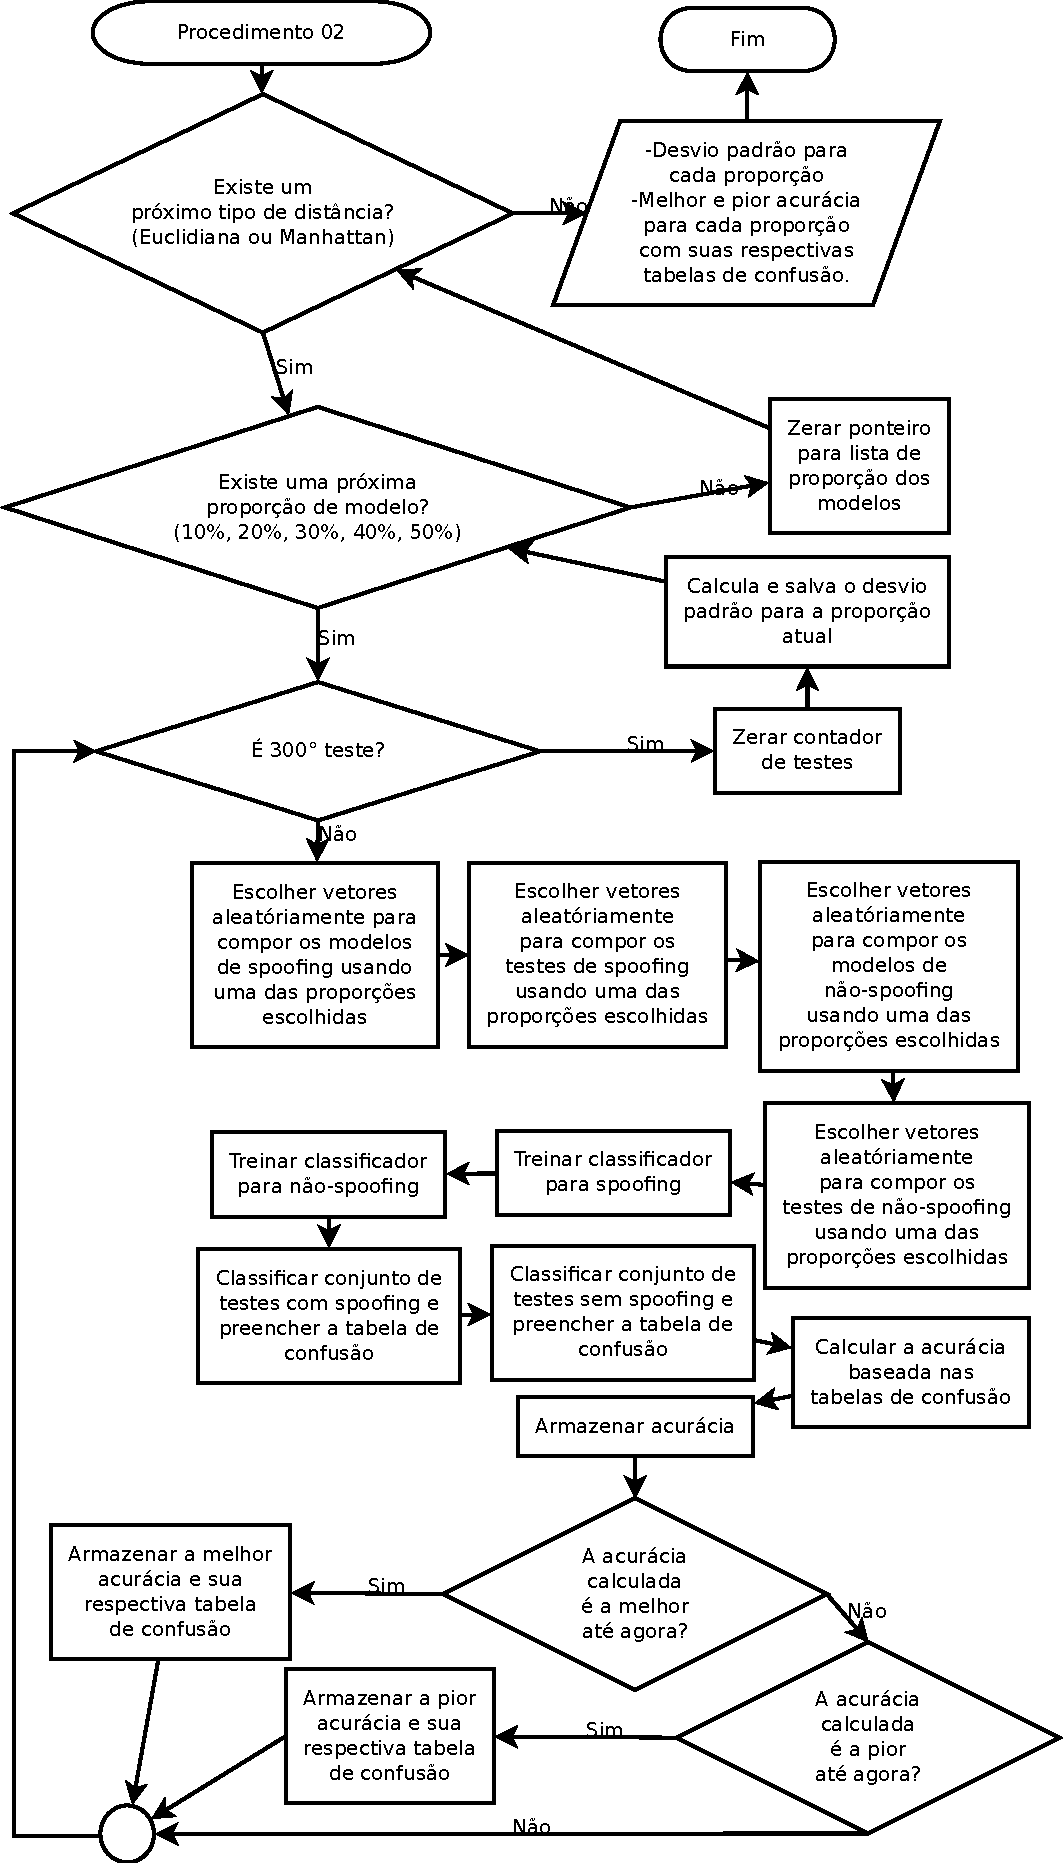
\includegraphics[angle=-90,width=1\linewidth]{images/AlgoProcedure02.pdf}
				\caption{Procedure 2 algorithm}
				\label{fig:experiment02Algo}
			\end{figure}
			
		\subsection{Procedure 3 - SVM classification}
			\label{sec:propApproach:subsec:Experiment3}

			\par Considering the best combinations discovered during procedure 1, this step aims to measure the accuracy of an SVM in classes separation. This classifier was chosen because previous studies prove its effectiveness for binary classification \cite{bennett2000support}. 
			
			\par In particular, the structure of the SVM used was defined as follows and according to Figure \ref{fig:3layersSVM}: 
			\begin{itemize}
				\item three layers, the first being the entrance, with passive elements, the second, with non-linear active elements of Gaussian nuclei and the third, that is, the exit, with a linear active element;

				\item there are no weights between the input layer and the intermediate layer, implying that the output of each input layer element connects with all the intermediate layer inputs, keeping the propagated values intact;
				
				\item the output of each intermediate layer element connects with the single element output layer through the weights $p_0, p_1, .... p_{X-1}$;

				\item the output value consists of the linear combination of the weights with the values received as input from the output layer, that is, the output values from the intermediate layer.
			\end{itemize}
			
			\begin{figure}
	\centering
	\scalebox{2}{
				\begin{tikzpicture}
	%input layer
	\node (input1) at (0.65,2.0) {};
	\draw[->,in=180,out=0] (1.0,2.0) to (1.35,2.0);
	\node (input2) at (0.65,1.5) {};
	\draw[->,in=180,out=0] (1.0,1.5) to (1.35,1.5);
	\node (input3) at (0.65,1.0) {};
	\draw[->,in=180,out=0] (1.0,1.0) to (1.35,1.0);
	\node (input3) at (0.65,0.0) {};
	\draw[->,in=180,out=0] (1.0,0.0) to (1.35,0.0);
	\node (IL_N1) at (1.5,2.0) {}; \filldraw[fill=gray!30] (1.5,2.0) circle (0.15cm);
	\node (IL_N2) at (1.5,1.5) {}; \filldraw[fill=gray!30] (1.5,1.5) circle (0.15cm);
	\node (IL_N3) at (1.5,1.0) {}; \filldraw[fill=gray!30] (1.5,1.0) circle (0.15cm);
	\node at (1.5,0.625) {$\vdots$};
	\node (IL_Nn) at (1.5,0.0) {}; \filldraw[fill=gray!30] (1.5,0.0) circle (0.15cm);
	
	%hidden layer 
	\node (HL_N1) at (3.5,2.5) {}; \filldraw[fill=blue!20] (3.55,2.5) circle (0.15cm);
	\node (HL_N2) at (3.5,2.0) {}; \filldraw[fill=blue!20] (3.55,2.0) circle (0.15cm);
	\node (HL_N3) at (3.5,1.5) {}; \filldraw[fill=blue!20] (3.55,1.5) circle (0.15cm);
	\node (HL_N4) at (3.5,1.0) {}; \filldraw[fill=blue!20] (3.55,1.0) circle (0.15cm);
	\node at (3.55,0.625) {$\vdots$};
	\node (HL_Nn-1) at (3.5,0.0) {}; \filldraw[fill=blue!20] (3.55,0.0) circle (0.15cm);	
	\node (HL_Nn) at (3.5,-0.5) {}; \filldraw[fill=blue!20] (3.55,-0.5) circle (0.15cm);	
	\draw[->,in=180,out=0] (IL_N1)+(1.5mm,0) to (HL_N1);
	\draw[->,in=180,out=0] (IL_N1)+(1.5mm,0) to (HL_N2);
	\draw[->,in=180,out=0] (IL_N1)+(1.5mm,0) to (HL_N3);
	\draw[->,in=180,out=0] (IL_N1)+(1.5mm,0) to (HL_N4);
	\draw[->,in=180,out=0] (IL_N1)+(1.5mm,0) to (HL_Nn-1);
	\draw[->,in=180,out=0] (IL_N1)+(1.5mm,0) to (HL_Nn);
	
	\draw[->,in=180,out=0] (IL_N2)+(1.5mm,0) to (HL_N1);
	\draw[->,in=180,out=0] (IL_N2)+(1.5mm,0) to (HL_N2);
	\draw[->,in=180,out=0] (IL_N2)+(1.5mm,0) to (HL_N3);
	\draw[->,in=180,out=0] (IL_N2)+(1.5mm,0) to (HL_N4);
	\draw[->,in=180,out=0] (IL_N2)+(1.5mm,0) to (HL_Nn-1);
	\draw[->,in=180,out=0] (IL_N2)+(1.5mm,0) to (HL_Nn);
	
	\draw[->,in=180,out=0] (IL_N3)+(1.5mm,0) to (HL_N1);
	\draw[->,in=180,out=0] (IL_N3)+(1.5mm,0) to (HL_N2);
	\draw[->,in=180,out=0] (IL_N3)+(1.5mm,0) to (HL_N3);
	\draw[->,in=180,out=0] (IL_N3)+(1.5mm,0) to (HL_N4);
	\draw[->,in=180,out=0] (IL_N3)+(1.5mm,0) to (HL_Nn-1);
	\draw[->,in=180,out=0] (IL_N3)+(1.5mm,0) to (HL_Nn);
	
	\draw[->,in=180,out=0] (IL_Nn)+(1.5mm,0) to (HL_N1);
	\draw[->,in=180,out=0] (IL_Nn)+(1.5mm,0) to (HL_N2);
	\draw[->,in=180,out=0] (IL_Nn)+(1.5mm,0) to (HL_N3);
	\draw[->,in=180,out=0] (IL_Nn)+(1.5mm,0) to (HL_N4);
	\draw[->,in=180,out=0] (IL_Nn)+(1.5mm,0) to (HL_Nn-1);
	\draw[->,in=180,out=0] (IL_Nn)+(1.5mm,0) to (HL_Nn);
	
	%output layer
	\node (OL_N1) at (5.5,1.0) {}; \filldraw[fill=red!40] (5.55,1.0) circle (0.15cm);
	
	\draw[->,in=180,out=0] (HL_N1)+(2mm,0) to (OL_N1);
	\draw[->,in=180,out=0] (HL_N2)+(2mm,0) to (OL_N1);
	\draw[->,in=180,out=0] (HL_N3)+(2mm,0) to (OL_N1);
	\draw[->,in=180,out=0] (HL_N4)+(2mm,0) to (OL_N1);
	\draw[->,in=180,out=0] (HL_Nn-1)+(2mm,0) to (OL_N1);
	\draw[->,in=180,out=0] (HL_Nn)+(2mm,0) to (OL_N1);
	%
	\draw[snake=brace,mirror snake,raise snake=45pt,brown] (1.25,1.25) -- (1.75,1.25) node[black,midway,yshift=-50pt,below]{\tiny camada de} node[black,midway,yshift=-58pt,below]{\tiny entrada com} node[black,midway,yshift=-66pt,below]{\tiny $R$ elementos}
	node[black,midway,yshift=-74pt,below]{\tiny passivos};
	\draw[snake=brace,mirror snake,raise snake=45pt,brown] (3.25,0.75) -- (3.75,0.75) node[black,midway,yshift=-50pt,below]{\tiny camada} node[black,midway,yshift=-58pt,below]{\tiny intermediária} node[black,midway,yshift=-66pt,below]{\tiny com $X$ neurônios}
	node[black,midway,yshift=-74pt,below]{\tiny ativos não-lineares};
	\draw[snake=brace,mirror snake,raise snake=45pt,brown] (5.25,1.75) -- (5.75,1.75) node[black,midway,yshift=-50pt,below]{\tiny camada de} node[black,midway,yshift=-58pt,below]{\tiny saída com} node[black,midway,yshift=-66pt,below]{\tiny um elemento}
	node[black,midway,yshift=-74pt,below]{\tiny ativo linear};
	%
	\node (OUT) at (6.5,1.0) {\tiny resultado}; 
	\draw[->,in=180,out=0] (OL_N1)+(2mm,0) to (OUT);	
	
	\node at (4,2.6) {\tiny $p_0$}; 
	\node at (4,2.1) {\tiny $p_1$}; 
	\node at (4,1.65) {\tiny $p_2$}; 
	\node at (4,1.2) {\tiny $p_3$}; 
	\node at (4,0.2) {\tiny $p_{X-2}$}; 
	\node at (4,-0.3) {\tiny $p_{X-1}$}; 
\end{tikzpicture}
	}
	\caption{Estrutura da SVM para o procedimento 03 com $R$ neurônios na camada de entrada, sendo $R$ a dimensão dos vetores de características, e $X$ neurônios na camada intermediária, sendo $X$ o número de casos de treinamento}
	\label{fig:3layersSVM}
\end{figure} 
			
			\par The number of elements in the input layer was equal to the feature vector dimension. In the intermediate layer, the number of active non-linear elements was equal to the number of training cases, aiming to facilitate the procedure that, in such a case, implies in the direct solution of a square linear system, that is, possible and determined \cite{poole2014linear}. 
			
			\par SVM training consists of, in an unsupervised first stage, adjusting the parameters of the Gaussian functions of the intermediate layer. Subsequently, based on the aforementioned linear system, the weights were found based on a supervised approach, using the labels -1 and 1 for the spoofed and genuine signals respectively.   
			
			\par All arrangements for the selection of training and testing vectors, as well as other details, are identical to those of procedure 2 and are listed in the Algorithm \ref{lst:experiment03Algo} and shown in Figure \ref{fig:experiment03Algo}. 
			
			\begin{lstlisting}[language=C++, caption={Algoritmo que caracteriza o procedimento 03}, label={lst:experiment03Algo}]
tamanhosDoModelo={0.1, 0,2, 0,4, 0,5};
modeloDeReferenciaNaoSpoofing={};
modeloDeReferenciaSpoofing={};
testesNaoSpoofing={};
testesSpoofing={};
	for(porcentagem : tamanhosDoModelo){
		for(teste = 0; teste < 300; teste++){
			// Escolhe aleatoriamente os sinais para o modelo com spoofing 
			// e os grava em 'modeloDeReferenciaSpoofing' o restante vai 
			// para 'testesSpoofing'
			escolherAleatoriamente(listaComVoiceSpoofing, porcentagem, modeloDeReferenciaSpoofing, testesSpoofing);
			
			// Escolhe aleatoriamente os sinais para o modelo sem spoofing
			// e os grava em 'modeloDeReferenciaNaoSpoofing' o restante vai 
			// para 'testesNaoSpoofing'
			escolherAleatoriamente(listaSemVoiceSpoofing, porcentagem, modeloDeReferenciaNaoSpoofing, testesNaoSpoofing);
			treinarClassificador("spoofing", modeloDeReferenciaSpoofing);
			treinarClassificador("naoSpoofing", modeloDeReferenciaNaoSpoofing);
			
			// Classifica os testes e preenche a tabela de confusao
			for(sinal : testesSpoofing){
				preencherTabelaDeConfusao(sinal, "spoofing");
			} 
			
			// Classifica os testes e preenche a tabela de confusao
			for(sinal : testesNaoSpoofing){
				preencherTabelaDeConfusao(sinal, "naoSpoofing");
			}
			
			acuracia=calculaAcuracia();
			
			// Salva a melhor acuracia e matriz de confusao
			if(ehAMelhorAcuracia(acuracia)){
				salvaAcuraciaEMatrizDeConfusao();
			}
			
			// Salva a pior acuracia e matriz de confusao
			if(ehAPiorAcuracia(acuracia)){
				salvaAcuraciaEMatrizDeConfusao();
			}
		}
	}			
\end{lstlisting}
			
			\begin{figure}[H]
				\centering
				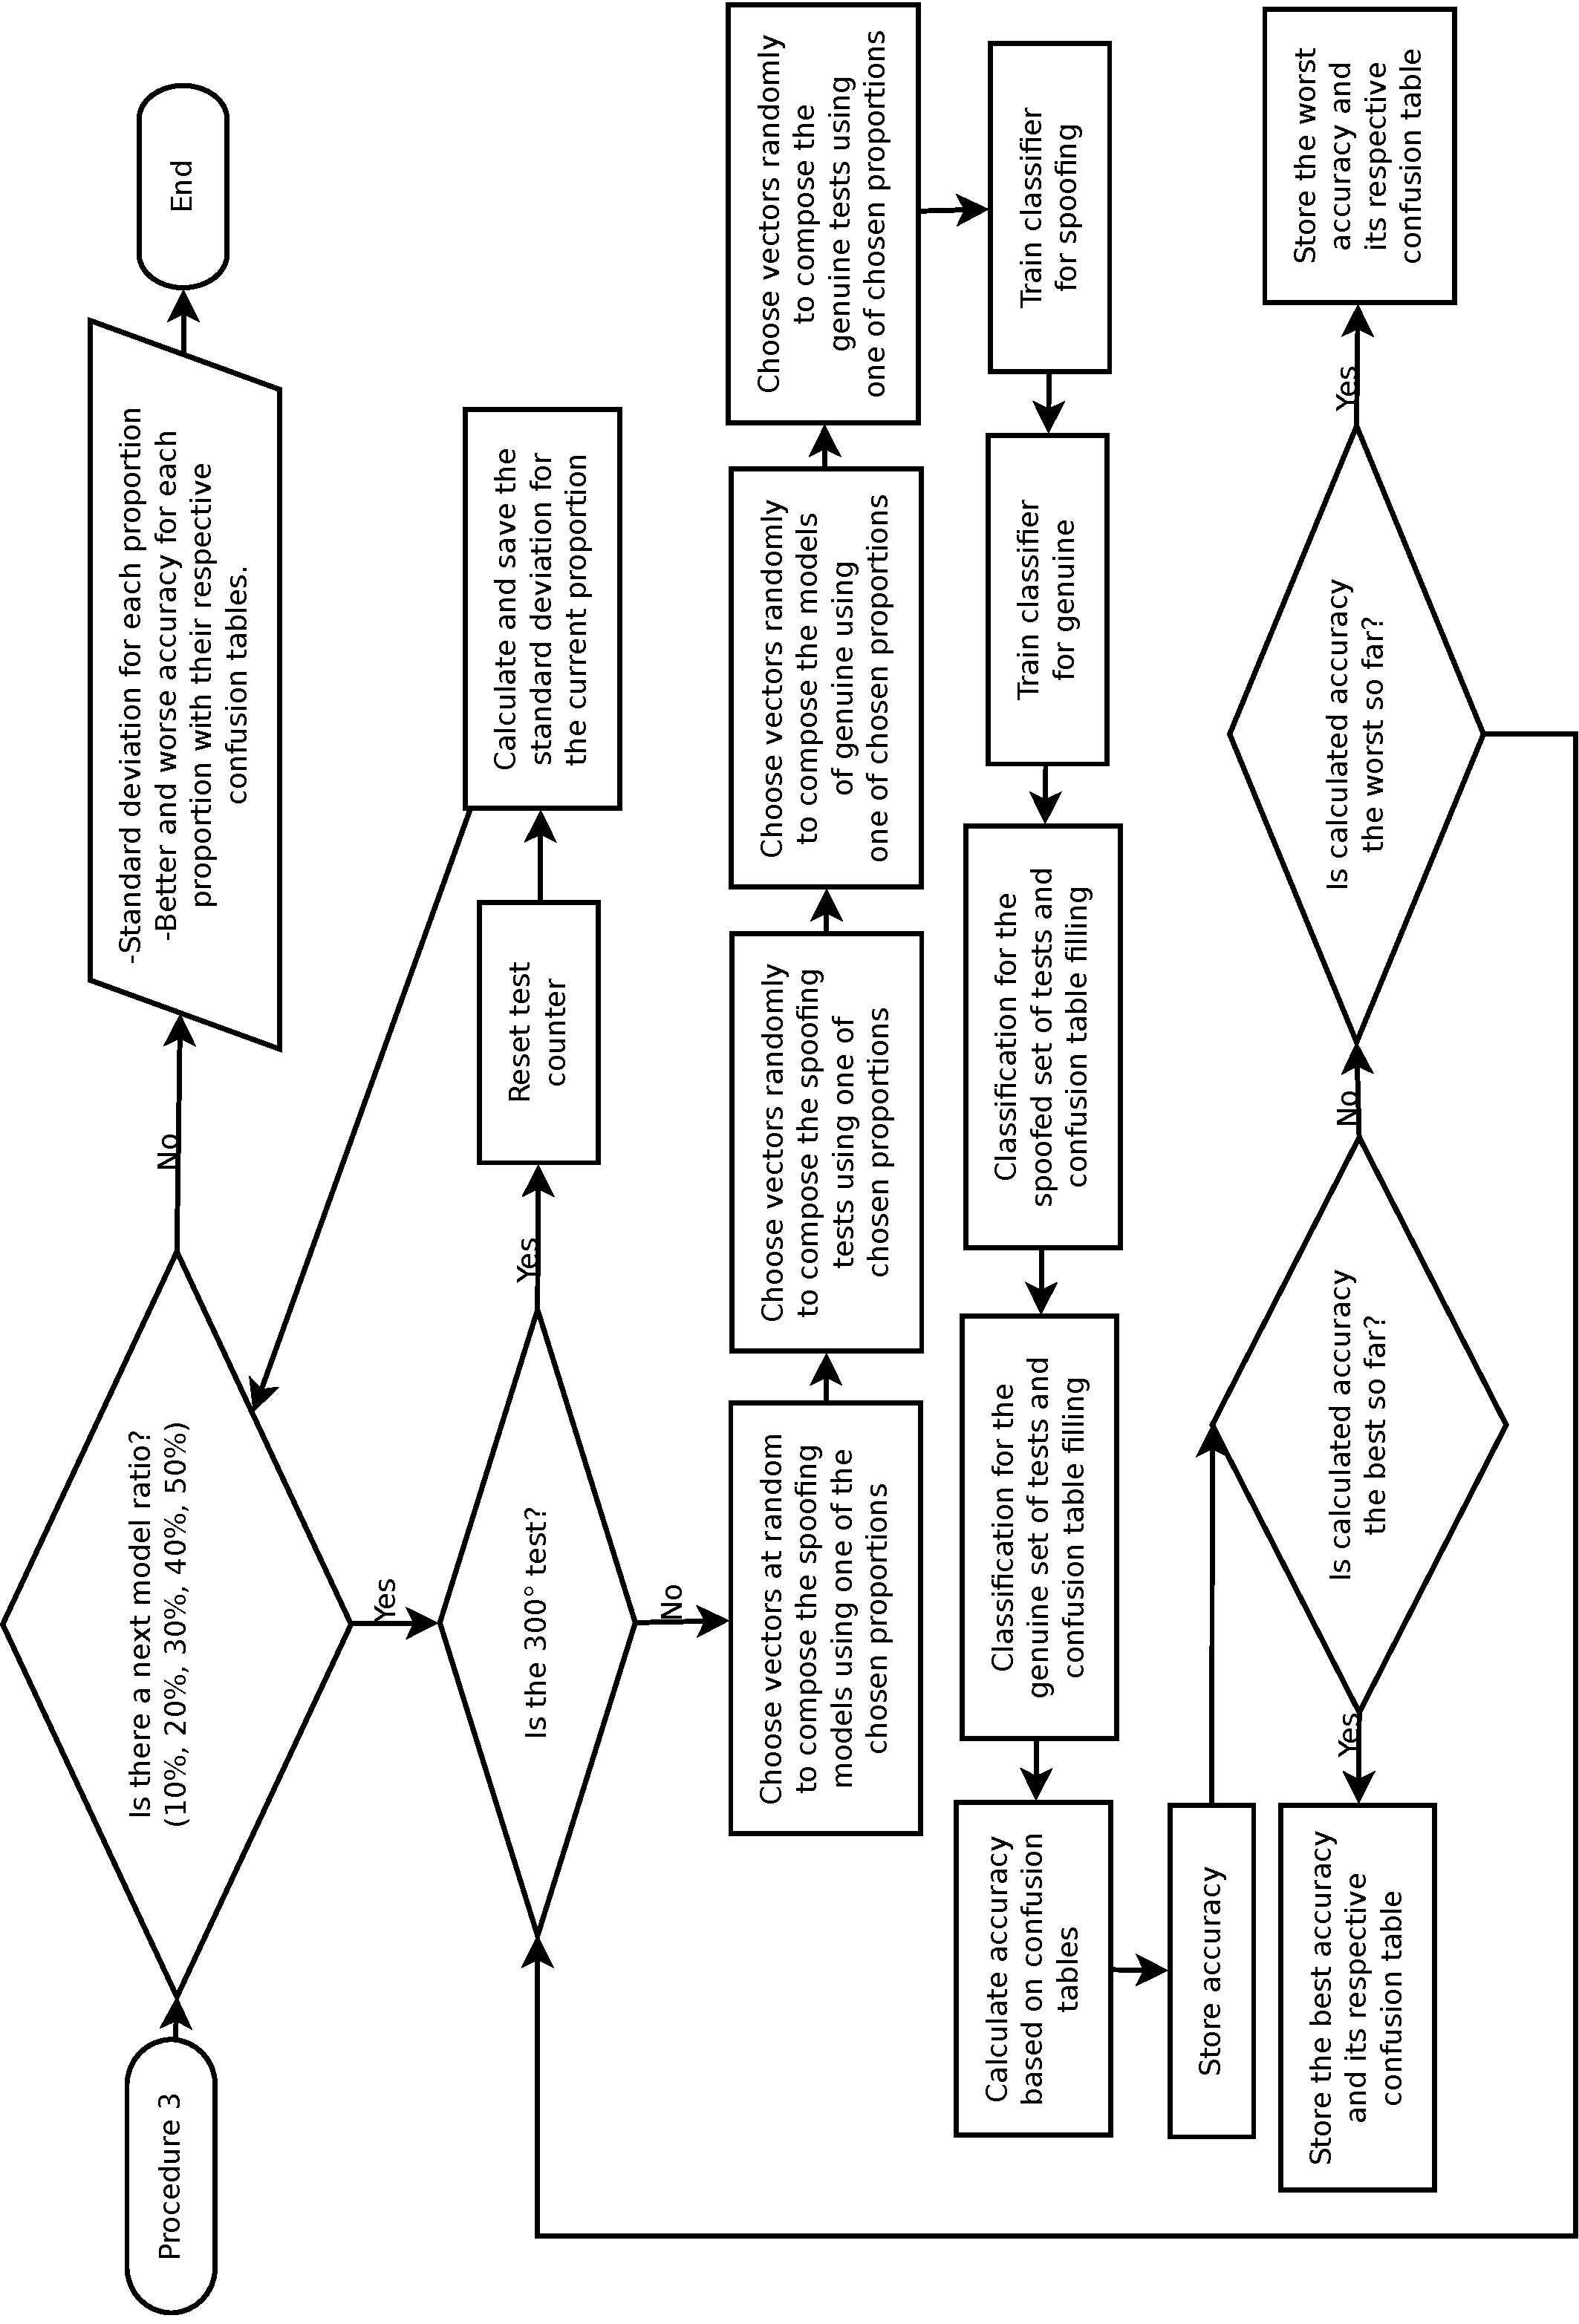
\includegraphics[angle=-90,width=1\linewidth]{images/AlgoProcedure03.pdf}
				\caption{Procedure 2 algorithm}
				\label{fig:experiment03Algo}
			\end{figure}
			
			\par The experiments tests and the results described in this Section are found in the next one.